\begin{figure}[h]
  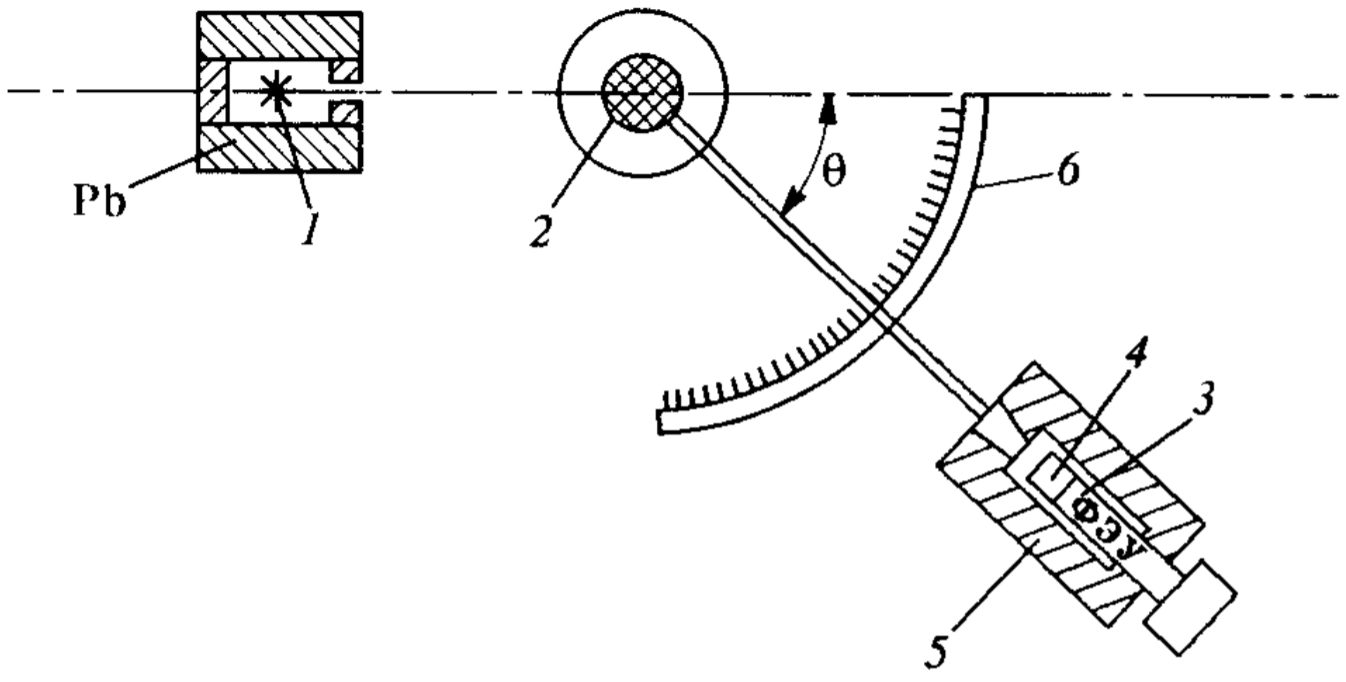
\includegraphics[width=0.7\textwidth]{2_1.png}
  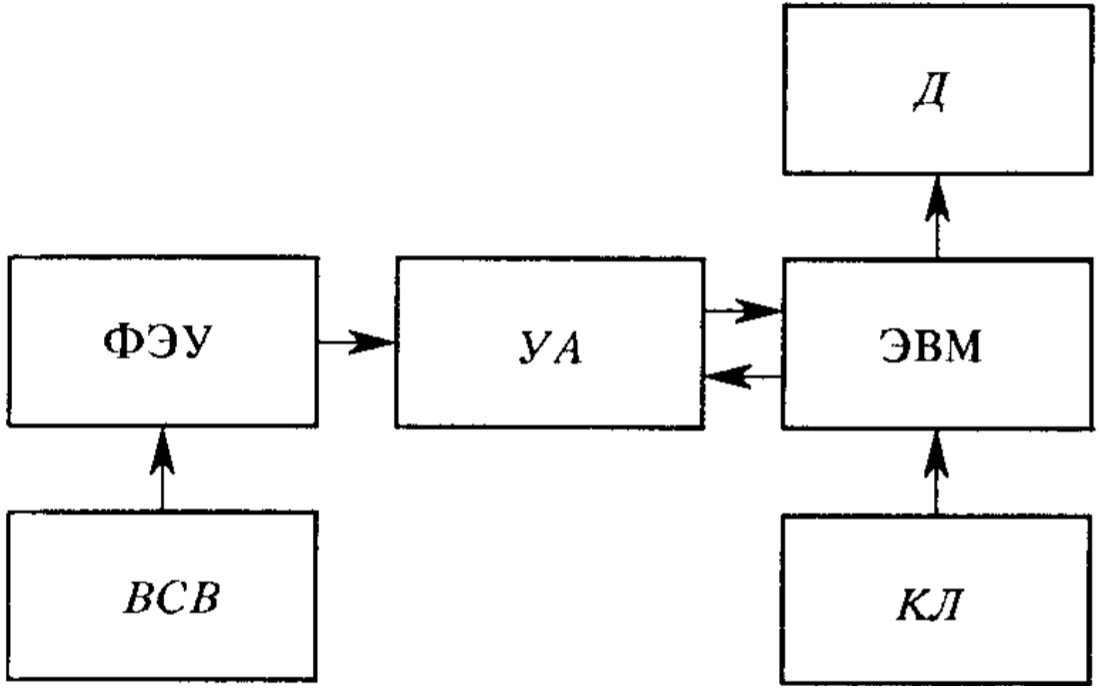
\includegraphics[width=0.7\textwidth]{2_2.png}
  \centering
  \caption{(a) Блок-схема установки по изучению рассеяния $\gamma$-квантов. (b) Блок-схема измерительного комплекса.}
  \label{Device}
\end{figure}

На рис. \ref{Device}а изображена блок-схема установки. Источником (1) служит
${}^{137}Cs$, испускающий $\gamma$-лучи с энергией $662$ кэВ, который помещён в
толстостенный свинцовый контейнер с коллиматором. Сформированный коллиматором
узкий пучок $\gamma$-квантов попадает на графитовую мишень (2), испытывает
рассеяние и регистрируется сцинтилляционным счётчиком, состоящим из
фотоэлектронного умножителя (ФЭУ) и сцинтиллятора -- выходное окно сцинтиллятора
находится в оптическом контакте с фотокатодом ФЭУ. Сигналы, возникающем в аноде
ФЭУ, подаются на компьютер для амплитудного анализа. Кристалл и ФЭУ расположены
в светонепроницаемом блоке, укреплённого на горизонтальной штанге, которая может
вместе с ним вращаться, угол поворота отсчитывается по лимбу (6). Головная часть
сцинтилляционного блока закрыта свинцовым коллиматором (5), который формирует
входной пучок и защищает детектор от постороннего излучения, в основном
$\gamma$-квантов, проходящих через стенки защитного контейнера источника. При
больших углах измерения для дополнительной защиты между контейнером и источником
и детектором ставился свинцовый экран.

\begin{figure}[h]
  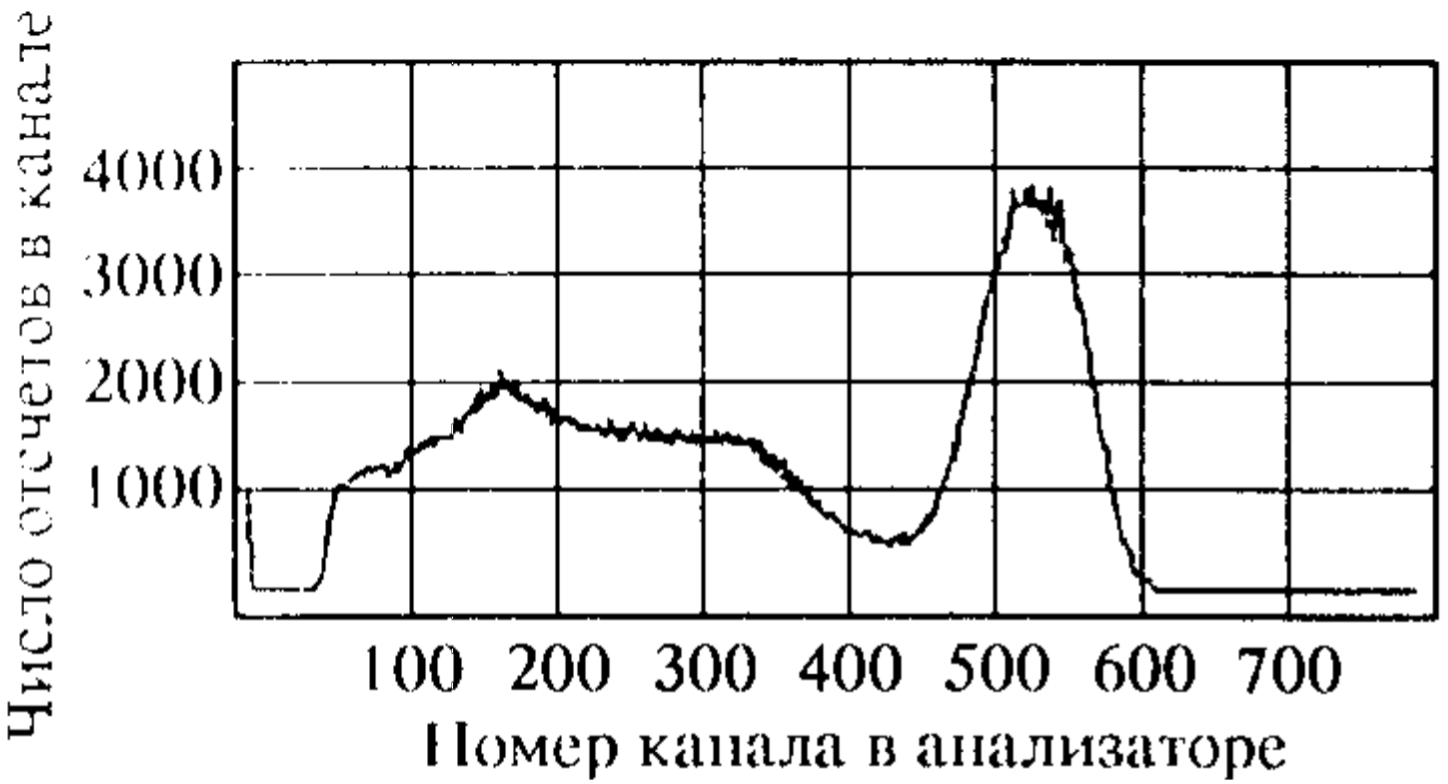
\includegraphics[width = 0.7\textwidth]{2_3.png}
  \centering
  \caption{Амплитудное распределение импульсов, возникающих в сцинтилляторе.}
  \label{Channel}
\end{figure}

Измерительный комплекс состоит из ФЭУ, питаемого от высоковольтного выпрямителя
ВСВ, усилителя-анализатора УА, являющегося входным интерфейсом компьютера ЭВМ,
управляемого с клавиатуры КЛ (рис. \ref{Device}b). Информация отображается на
дисплее Д. При работе ФЭУ в спектрометрическом режиме величина выходного
электрического импульса пропорциональна энергии регистрируемого $\gamma$-кванта.
В итоге возникает распределение электрических импульсов (рис. \ref{Channel}),
имеющее фотопик, положение вершины которого нас будет интересовать. Левее
фотопика начинается непрерывный спектр комптоновских электронов, который
сохраняется при любом угле рассеяния. Номер канала на распределении
соответствует энергии регистрируемой частицы, точность его определения примерно
$1\%$.


Пусть $\varepsilon(\theta) = AN(\theta)$, $A$ -- коэффициент пропорциональность,
$N(\theta)$ -- номер соответствующего канала. Тогда \eqref{Eps} перепишется как
\[\tag{1b}\label{1b} \dfrac{1}{N(\theta)} - \dfrac{1}{N(0)} = A(1-\cos
  \theta).\] Отсюда можно определить энергию покоя электрона как

\begin{equation}\label{2}
  mc^2 = E_\gamma \dfrac{N(90)}{N(0) - N(90)},
\end{equation}
\\
где $E_\gamma = E_0$ -- энергия испускаемых источником $\gamma$-квантов.

